\documentclass{article}
\usepackage[utf8]{inputenc}
\setlength{\parskip}{1.5em}
\setlength\parindent{24pt}
\usepackage{graphicx}
\graphicspath{ {./images/} }
\title{\vspace{-2.0cm}A Probabilistic Analysis of the Homogenous Isotropic Waldo Localization Distribution in an N Dimensional Topological Space}
\author{William Tom}
\date{}
\usepackage{amsmath, amsthm, amssymb, amsfonts}
\usepackage{siunitx}
\usepackage{graphicx}
\usepackage{color}
\usepackage{physics}
\usepackage{hyperref}
\hypersetup{
    colorlinks=true,
    linkcolor=blue,
    filecolor=magenta,      
    urlcolor=blue,
}
\begin{document}
\maketitle
\section{Introduction}
The \emph{Where's Waldo?}, or \emph{Where's Wally?} books, originally published in 1987,\footnote{Waldo Wiki, "Where's Waldo?"} are a series of puzzle books. The books consist of heavily detailed cartoon images drawn onto a double-page spread, depicting a large number of objects and people in various locations performing a variety of comical actions. These locations might include, but are not limited to the beach, a movie theatre, a medieval town, or the "Land of Woofs." The central task for the reader is then to locate the titular character, Waldo.\footnote{It's worth noting that there exist other recurring characters. However, this analysis chiefly concerns the properties of Waldo.}
\begin{center}
	
\includegraphics[scale=.1]{waldo.png}\\
	\emph{Figure 1:} Waldo, depicted in his standard red-and-white striped outfit, bobble hat, and glasses.\footnote{Twitter, "Where's Waldo?"}
\end{center}
However, this is no simple task. The book is intentionally designed to be deceptive, with Waldo's distinctive outfit hidden beneath numerous similar objects and people meant to misdirect your attention. Hence, the challenge of finding Waldo has repeatedly stumped the minds of children and academics alike. 

In this paper, we seek to determine the distribution of Waldo's spatial localization. To this end, we must also classify the nature of Waldo, as well as the space within which he exists. The solution to this problem lies in a probabilistic analysis of his localization and considering a variety of subjects, from topology to quantum mechanics. We believe this will be useful to scientists across the world, answering Waldo-related questions many of us have had since childhood. In the future, our research can be extended to the variety of other characters in the \emph{Where's Waldo} series, as well as any similar books.

\section{The Topology of Waldo}
A description of Waldo's localization would be incomplete without a prior examination of Waldo's topology. As posited by Adjunct Professor Dahl in his paper on the subject, Waldo can be thought to occupy 4 dimensional Minkowski space.\footnote{Dahl, "Roald Dahl on Writing."} However, this has been shown to be non-homeomorphic to model spaces suggested by experiment. Hence, we must first determine any relevant topological properties.

While an analysis rooted solely in phase space seems initially promising, this fails to give accurate results when compared to experimental evidence. Instead, we consider a system of multiple $\mathbb{R}_+^{2}$, or the quotient space given by
\begin{equation}
	\mathcal{W} = \sqcup^N_{\substack{k=1}} \mathbb{R}^2_+ / \mathbb{R}.
\end{equation}
\begin{center}
	
\includegraphics[scale=.1]{waldospace.png}\\
	\emph{Figure 2:} An embedding of such a system in real Euclidean space.
\end{center}
Not only does this model provide accurate results, it also allows us to treat each $\mathbb{R}_+^{2}$ separately. This provides the manifold properties imperative to Waldo's localization, including the introduction of a Euclidean metric, and  hence we will call each sheet of the space a \emph{Waldofold.}
\begin{center}
	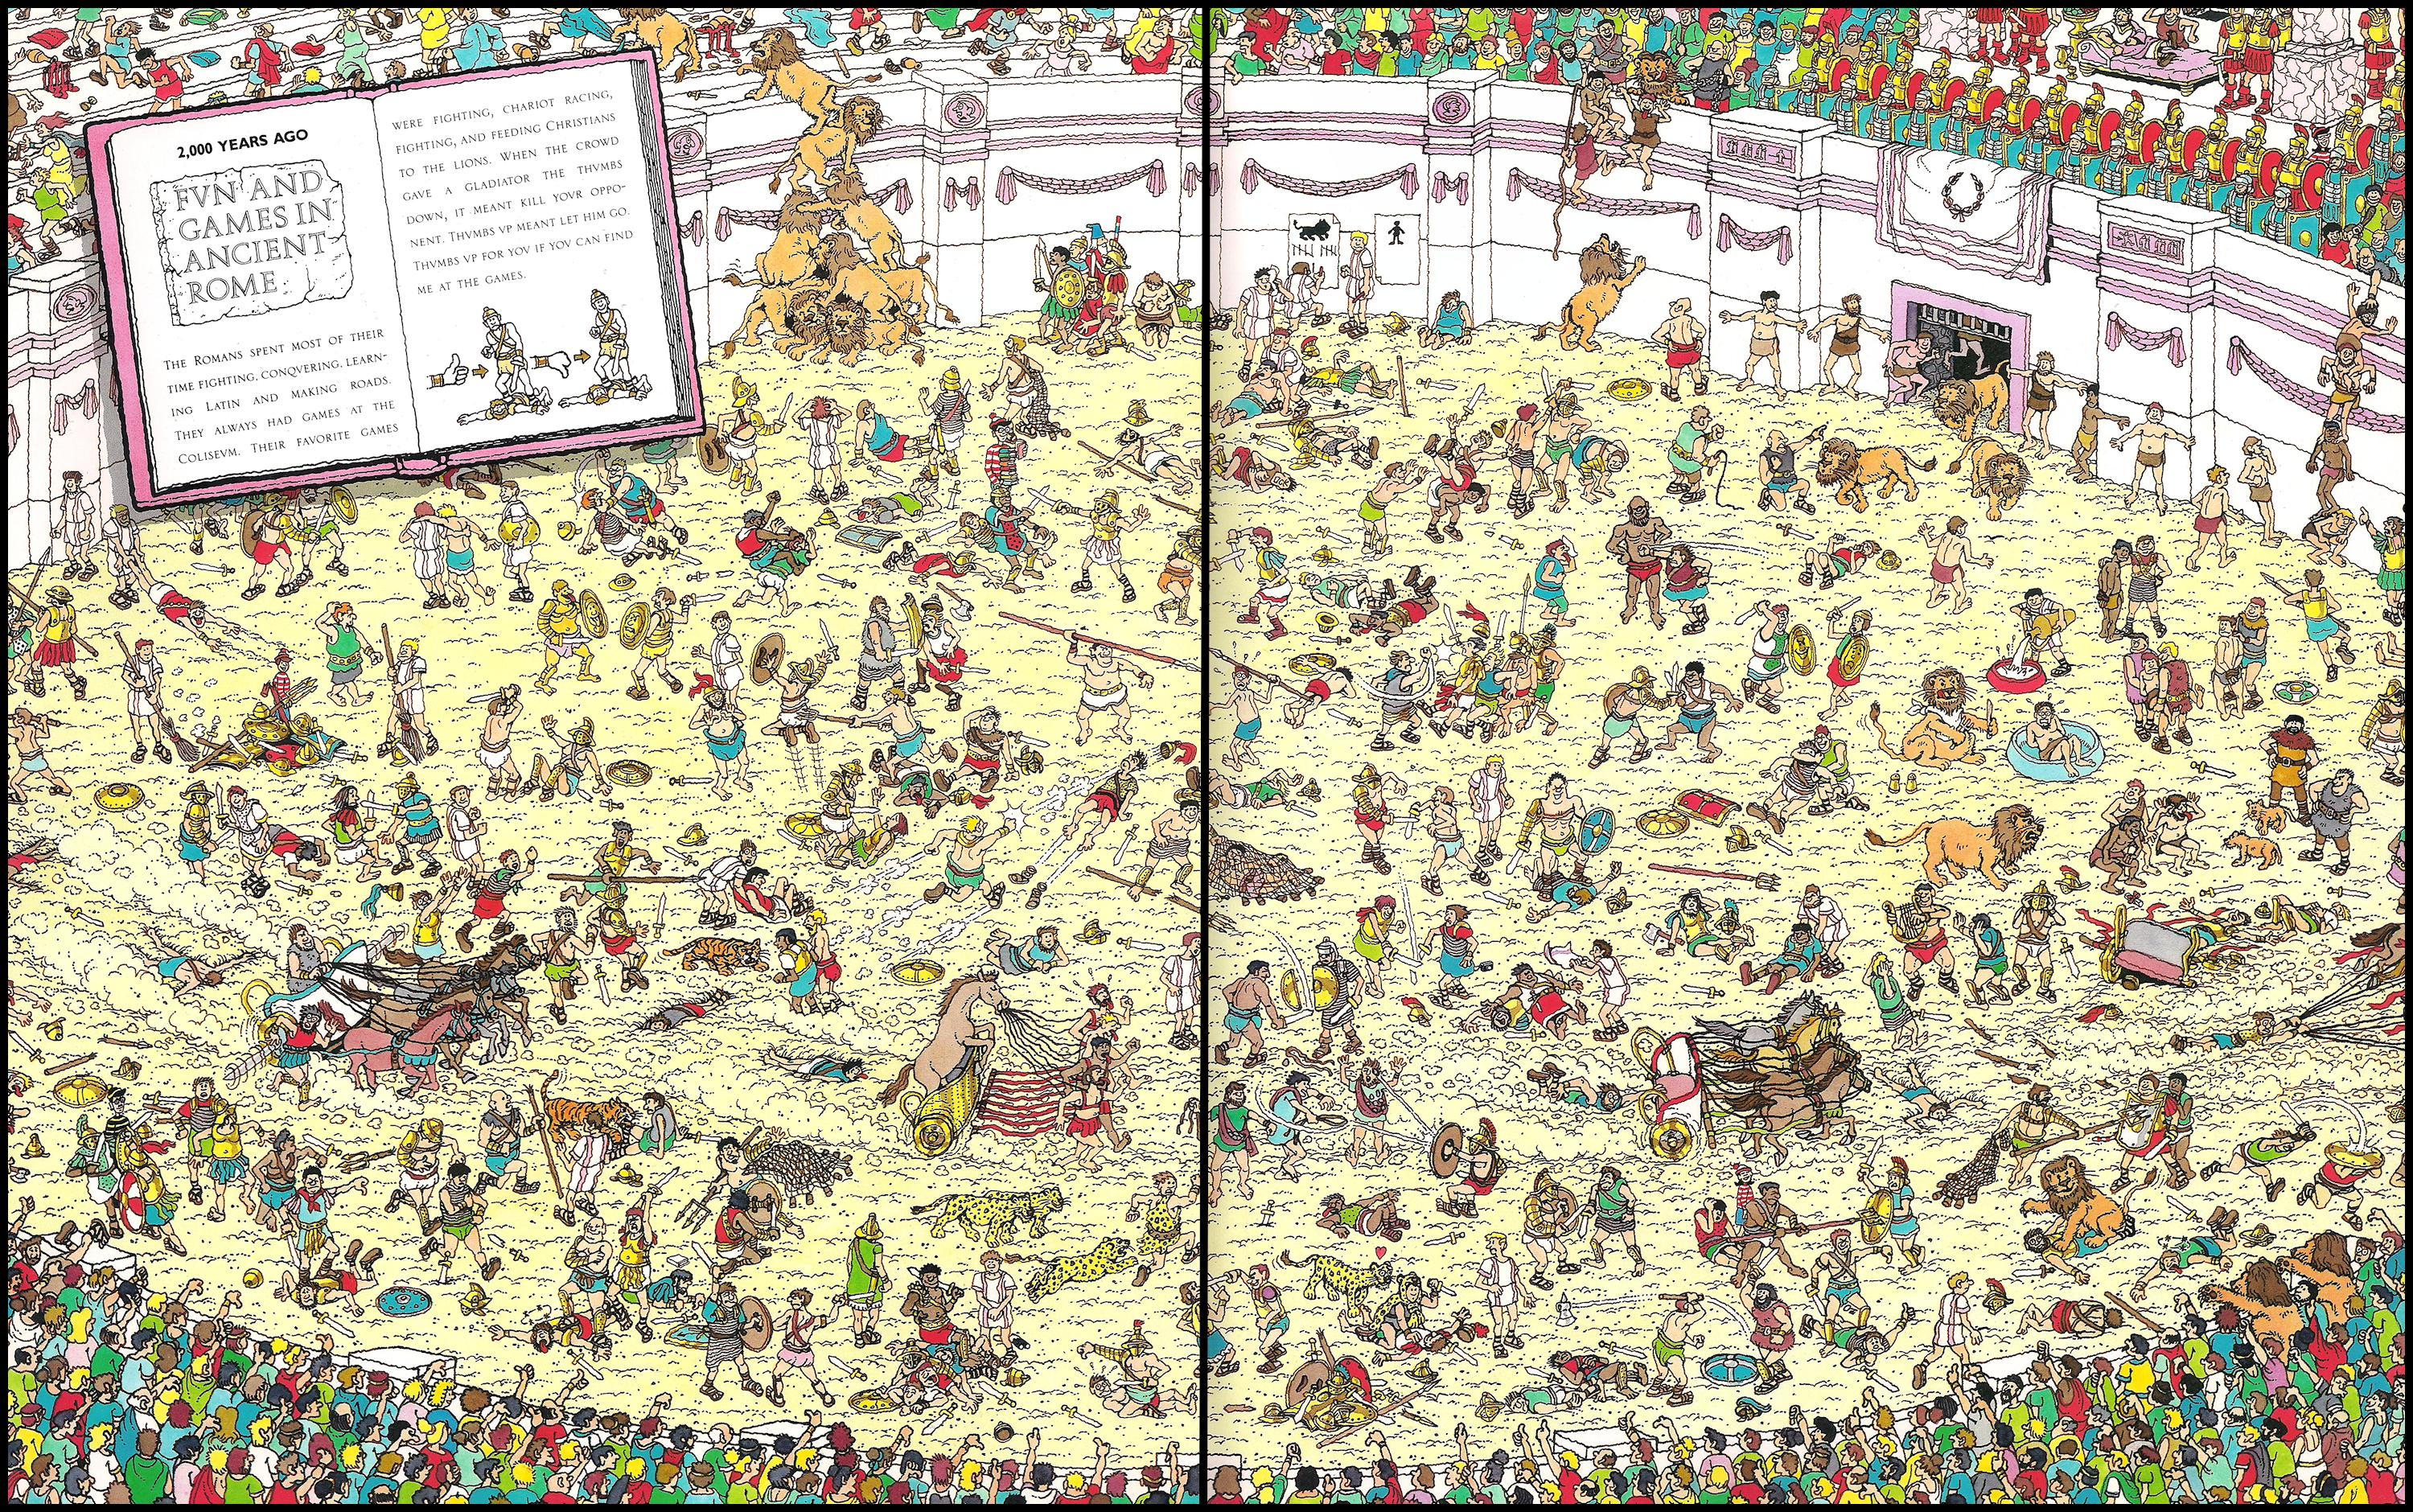
\includegraphics[scale=.1]{waldofold.jpg}\\
\emph{Figure 3:} An example of two Waldofolds connected along $\mathbb{R}$.
\end{center}
\section{The Quantum Mechanical Properties of Waldo}
Having determined a suitable space within which to perform calculations, we quickly realize that a deterministic view of Waldo's location on a Waldofold is impossible. Therefore, we instead consider a probabilistic view, hence a Waldo localization distribution. Assuming Waldo is regularly sized, and small compared to each Waldofold, we can invoke the \emph{Small Waldo Approximation.} This tells us that, when compared to the whole Waldofold, Waldo acts approximately like a particle, and will henceforth be treated as such. Borrowing from quantum mechanics, we apply the Schrödinger Equation,
\begin{equation}
	-\frac{\hbar^2}{2m}\grad_2^2\psi(x,y,t)+V(x,y)\psi(x,y,t) = i\hbar\frac{\partial\psi(x,y,t)}{\partial t}.
\end{equation}
Once again invoking the Small Waldo Approximation, and assuming that Waldofolds are isotropic and homogenous up to action by $K_4$, we notice that a single Waldofold resembles an infinite square well. The standard solution yields eqns. \ref{eq:3}, \ref{eq:4}, the proof of which is left to the reader.
\begin{equation}
	\label{eq:3}
	\psi(x,y,t) = \frac{\sqrt{2}}{\sqrt{L_xL_y}}\sin\Big(\frac{n_x \pi x}{L_x}\Big)\sin\Big(\frac{n_y \pi y}{L_y}\Big)e^{\frac{-iEt}{\hbar}}
\end{equation}
\begin{equation}
	\label{eq:4}
	E = \Big(\frac{n^2_x}{L^2_x}+\frac{n^2_y}{L^2_y}\Big)\frac{(hc)^2}{8mc^2}
\end{equation}
Having obtained our Waldofunction, we now perform the usual manipulations to calculate the localization distribution within a Waldofold.
\begin{equation}
	\label{eq:5}
	|\psi(x,y)|^2 = \sin^2 \Big(\frac{n_x \pi x}{L_x} \Big) \sin^2 \Big(\frac{n_y \pi y}{L_y} \Big)
\end{equation}
Evaluating eqn. \ref{eq:5} for the standard Waldofold dimensions of $2.5908 \cross 10^8 \si{\nano\metre}$ by $3.175 \cross 10^8 \si{\nano\metre}$\footnote{Handford, "Where's Waldo?: Deluxe Edition: Hardcover."} gives, for a single Waldofold,
\begin{equation}
	\label{eq:6}
	\mathcal{P}(\text{Waldofold}) = \frac{1}{2}.
\end{equation}
Therefore the probability of finding Waldo on any given Waldofold is $\frac{1}{2}$. This same analysis can be extended to Waldo's girlfriend, Wenda, both by the method detailed and by naturally extending the Poisson Distribution to a Waldofold through diffeomorphic continuation; however, this is trivial and will not be discussed further. Interestingly, neither method works for any of the other characters.
\begin{center}
	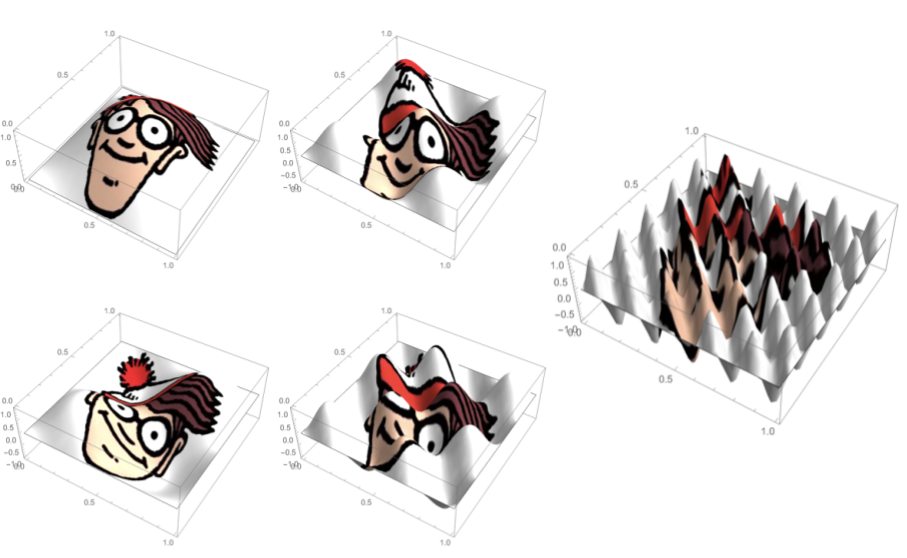
\includegraphics[scale=.4]{graphs.png}\\
	\emph{Figure 4:} The Waldofunction evaluated with $L_{x,y} = 1$, neglecting the preceding constant and phase. \\Top Row: $n_{x,y} = 1$, $n_{x,y} = 2$ Bottom Row: $n_{x,y} = 3$, $n_{x,y} = 4$ \\Right: $n_{x,y} = 10$.	
\end{center}
\section{Further Work}
In this paper, we have presented an explanation for Waldo's localization distribution in an arbitrarily dimensioned quotient space, and derived certain results using standard quantum theory. Namely, the probability of finding Waldo on any given Waldofold is $.5$.  This is an interesting result, as it does not guarantee that Waldo is on any given double-page spread. Instead, it suggests a probability of $.5$ for finding Waldo in any given page, and hence a probability of $1-.5^{32}$ for any given book, using an average length of 32 pages. Why is this the case? Is it simply a wonder of probability that we manage to find a Waldo on every double page spread? Or is the universe occupied by "anti-Waldos" of sorts, taking into account our overmeasuring of Waldo population? These questions require further testing and exploration. Additionally, our research can be extended to the variety of other Where's Waldo characters, such as Odlaw, Woof, and Wizard Whitebeard. For the time being, however, it's safe to say that Waldo has indeed been found, and the scientific community can finally resume progress in other fields.
\section{References}
\begin{enumerate}
	\item "Where's Waldo?" Waldo Wiki. Accessed October 27, 2020. \\\href{https://waldo.fandom.com/wiki/Where's_Waldo?}{https://waldo.fandom.com/wiki/Where's\_Waldo?}
	\item "Where's Waldo?" Twitter. Accessed October 27, 2020. \\\href{https://twitter.com/whereswaldo}{https://twitter.com/whereswaldo}.
	\item Dahl, Roald. "Roald Dahl on Writing." Accessed October 29, 2020. \href{https://www.roalddahl.com/create-and-learn/write/roald-dahl-on-writing}{https://www.roalddahl.com/create-and-learn/write/roald-dahl-on-writing}.
	\item Handford, Martin. "Where's Waldo?: Deluxe Edition: Hardcover." Barnes \& Noble. August 14, 2012. Accessed October 27, 2020. \href{https://www.barnesandnoble.com/w/wheres-waldo-handford-martin/1112764849}{\\https://www.barnesandnoble.com/w/wheres-waldo-handford-martin/1112764849}. 
\end{enumerate}
\end{document}
